\documentclass[11pt, a4paper]{article}
\usepackage[T1]{fontenc}
\usepackage[utf8]{inputenc}
\usepackage{lmodern}
\usepackage[margin=2cm, top=2.5cm, bottom=2.5cm, headheight=14pt]{geometry}
\usepackage{amsmath}
\usepackage{amssymb}
\usepackage[table]{xcolor}
\usepackage{tikz}
\usetikzlibrary{calc}
\usepackage{tcolorbox}
\tcbuselibrary{breakable}
\usepackage{tabularx}
\usepackage{booktabs}
\usepackage{enumitem}
\usepackage{parskip}
\usepackage{titlesec}
\usepackage{fancyhdr}

%— Colours
\definecolor{accent}{RGB}{22,163,74}
\definecolor{accentlight}{RGB}{240,253,244}
\definecolor{accentmid}{RGB}{34,197,94}
\definecolor{errred}{RGB}{220,38,38}
\definecolor{errbg}{RGB}{254,242,242}
\definecolor{orng}{RGB}{249,115,22}
\definecolor{orngbg}{RGB}{255,247,237}
\definecolor{retreival}{RGB}{29,78,216}
\definecolor{retrievalbg}{RGB}{239,246,255}
\definecolor{slate}{RGB}{71,85,105}
\definecolor{slatelight}{RGB}{148,163,184}
\definecolor{dblue}{RGB}{29,78,216}

%— Headings
\titleformat{\section}{\large\bfseries\color{accent}}{}{0em}{}[\color{accentmid}\titlerule]
\titleformat{\subsection}{\normalsize\bfseries\color{slate}}{}{0em}{\MakeUppercase}
\titlespacing{\section}{0pt}{18pt}{8pt}
\titlespacing{\subsection}{0pt}{14pt}{4pt}

%— Helpers
\newcommand{\blank}[1]{\underline{\hspace{#1}}}
\newcommand{\dgr}{\ensuremath{^\circ}}
\newcommand{\answerline}{\par\vspace{0.45cm}\noindent\rule{\linewidth}{0.4pt}\par\vspace{0.1cm}}
\newcommand{\selfcheck}{\par\smallskip\noindent\textbf{Self-check:}
  $\square$~I could teach it\quad$\square$~Getting there\quad$\square$~Not yet\smallskip}

%— tcolorbox styles
\tcbset{
  misconc/.style={colback=errbg,colframe=errred,
    title={\small\bfseries\color{errred}Misconception},
    left=6pt,right=6pt,top=3pt,bottom=3pt,breakable},
  worked/.style={colback=accentlight,colframe=accentmid,
    fonttitle={\small\bfseries\color{accent}},
    left=6pt,right=6pt,top=3pt,bottom=3pt,breakable},
  retrieval/.style={colback=retrievalbg,colframe=dblue!40,
    title={\small\bfseries\color{retreival}Retrieval Check --- \textit{Close your notes}},
    left=6pt,right=6pt,top=3pt,bottom=3pt,breakable},
  connection/.style={colback=orngbg,colframe=orng,
    left=6pt,right=6pt,top=3pt,bottom=3pt,breakable},
  learningtarget/.style={colback=accentlight,colframe=accentmid,
    leftrule=3pt,toprule=0pt,bottomrule=0pt,rightrule=0pt,
    left=8pt,right=6pt,top=3pt,bottom=3pt},
  preknowledge/.style={colback=gray!5,colframe=gray!30,
    left=8pt,right=8pt,top=6pt,bottom=6pt,breakable}
}

%— TikZ circle vocabulary diagram (reused twice)
\newcommand{\circlevocabdiagram}{%
\begin{center}
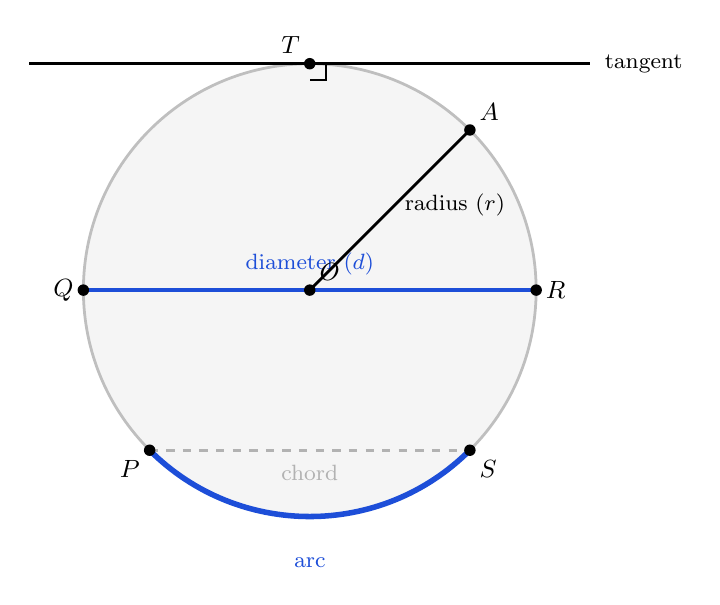
\begin{tikzpicture}[scale=1.15, font=\small]
  % Points
  \coordinate (O) at (0,0);
  \coordinate (T) at (0,2.5);
  \coordinate (Q) at (-2.5,0);
  \coordinate (R) at (2.5,0);
  \coordinate (A) at (1.768,1.768);   % 45 deg
  \coordinate (P) at (-1.768,-1.768); % 225 deg
  \coordinate (S) at (1.768,-1.768);  % 315 deg
  % Circle
  \draw[gray!50, fill=gray!8, line width=1pt] (O) circle (2.5);
  % Tangent line at T
  \draw[line width=1pt] (-3.1,2.5) -- (3.1,2.5);
  % Right-angle mark at T
  \draw[line width=0.8pt] (0.18,2.5)--(0.18,2.32)--(0,2.32);
  % Diameter Q-R
  \draw[dblue, line width=1.6pt] (Q)--(R);
  \node[dblue, above, yshift=2pt] at (0,0) {\footnotesize diameter ($d$)};
  % Radius O-A
  \draw[line width=1pt] (O)--(A);
  \node[right, xshift=2pt, yshift=2pt] at (0.88,0.88) {\footnotesize radius ($r$)};
  % Chord P-S (dashed)
  \draw[gray!60, dashed, line width=1pt] (P)--(S);
  \node[gray!60, below, yshift=-2pt] at (0,-1.768) {\footnotesize chord};
  % Minor arc P to S through bottom (225 -> 315)
  \draw[dblue, line width=2pt] (P) arc (225:315:2.5);
  \node[dblue, below] at (0,-2.85) {\footnotesize arc};
  % Point markers
  \foreach \pt in {O,T,Q,R,A,P,S}
    \fill (\pt) circle (1.8pt);
  % Labels
  \node[above right] at (O) {$O$};
  \node[above left]  at (T) {$T$};
  \node[left]        at (Q) {$Q$};
  \node[right]       at (R) {$R$};
  \node[above right] at (A) {$A$};
  \node[below left]  at (P) {$P$};
  \node[below right] at (S) {$S$};
  % Tangent label
  \node[right] at (3.15,2.5) {\footnotesize tangent};
\end{tikzpicture}
\end{center}}

%— Header / footer
\pagestyle{fancy}
\fancyhf{}
\fancyhead[L]{\small\color{slate}Circle Geometry --- Grade 9 Mathematics}
\fancyhead[R]{\small\color{slate}Alberta Curriculum}
\fancyfoot[C]{\small\color{slatelight}\thepage}
\renewcommand{\headrulewidth}{0.4pt}
\renewcommand{\headrule}{\color{slatelight}\hrule width\headwidth height\headrulewidth}

% ═══════════════════════════════════════════════════
\begin{document}
% ═══════════════════════════════════════════════════

%— Title block
\begin{tcolorbox}[colback=accentlight, colframe=accent, leftrule=5pt,
    toprule=0.6pt, bottomrule=0.6pt, rightrule=0.6pt,
    top=8pt, bottom=8pt, left=12pt]
  {\small\bfseries\color{accent}GRADE 9 MATHEMATICS
    \textperiodcentered{} ALBERTA CURRICULUM
    \textperiodcentered{} MEASUREMENT \& GEOMETRY}\\[4pt]
  {\LARGE\bfseries Circle Geometry}\\[3pt]
  {\small\color{slate}Guided Notes Package}
\end{tcolorbox}

\vspace{6pt}
\noindent Name:\;\blank{6cm}\hfill Date started:\;\blank{4cm}
\vspace{14pt}

% ───────────────────────────────────────────────────
\section*{Pre-Knowledge Check}

\begin{tcolorbox}[preknowledge]
\textit{No marks. No correction. Be honest --- write exactly what you think right now.}

\vspace{6pt}
Label any parts of a circle that you already know on this diagram:

\circlevocabdiagram

What do you think an ``inscribed angle'' is? Make your best guess.
\answerline

What angle do you think is formed when a radius meets the edge of a circle?
\answerline

\textit{You will come back to this page at the end of the unit. Do not erase your answers.}
\end{tcolorbox}

\clearpage

% ───────────────────────────────────────────────────
\section{Section 1 --- Circle Vocabulary}

\begin{tcolorbox}[learningtarget]
\small\textit{\textbf{Learning target:} I can identify and name all major parts of a circle and use precise geometric language when describing circle relationships.}
\end{tcolorbox}

\subsection{Vocabulary}

\renewcommand{\arraystretch}{1.9}
\begin{tabularx}{\linewidth}{|p{3.3cm}|X|X|}
\hline
\rowcolor{accentlight}\textbf{Term} & \textbf{Definition in your own words} & \textbf{One example / drawing} \\
\hline
Centre    & & \\ \hline
Radius    & & \\ \hline
Diameter  & & \\ \hline
Chord     & & \\ \hline
Arc       & & \\ \hline
Central angle  & & \\ \hline
Inscribed angle & & \\ \hline
Tangent        & & \\ \hline
Point of tangency & & \\ \hline
Semicircle     & & \\ \hline
\end{tabularx}
\renewcommand{\arraystretch}{1}

\subsection{Guided Notes}

\textbf{Label each part on the diagram below:}

\circlevocabdiagram

Fill in the labels: P, Q, O, R, T, and the two unlabelled lines.

\vspace{6pt}
\textbf{Fill in the blanks:}

The \textbf{centre} of a circle is the point \blank{4.5cm} from all points on the circle.

The \textbf{radius} ($r$) goes from the \blank{3cm} to any point on the circle.

The \textbf{diameter} ($d$) is the \blank{3cm} chord --- it passes through the \blank{3cm}.

\[d = \underline{\phantom{XX}} \times r \qquad\qquad r = d \div \underline{\phantom{XX}}\]

A \textbf{chord} is a line segment with both endpoints on the \blank{4cm}. \textit{(The diameter is a special chord.)}

An \textbf{arc} is \blank{5cm} of the circle between two points.

\begin{tcolorbox}[misconc]
\textbf{Wrong idea:} ``Any chord that goes through the circle is a diameter.''

\smallskip
\textbf{Why it fails:} A diameter is a chord that passes specifically through the \textit{centre}. Most chords do not pass through the centre and are shorter than the diameter. Every diameter is a chord, but not every chord is a diameter.

\smallskip
In the diagram above, QR passes through the centre O, so QR is a \blank{3cm}.\newline
A chord that does not pass through O would be \blank{3cm} the diameter.
\end{tcolorbox}

\textbf{Central angle vs.\ inscribed angle:}

A \textbf{central angle} has its vertex at the \blank{3.5cm} of the circle.

An \textbf{inscribed angle} has its vertex on the \blank{3.5cm} of the circle, with both sides being chords.

Draw an example of each:

\begin{center}
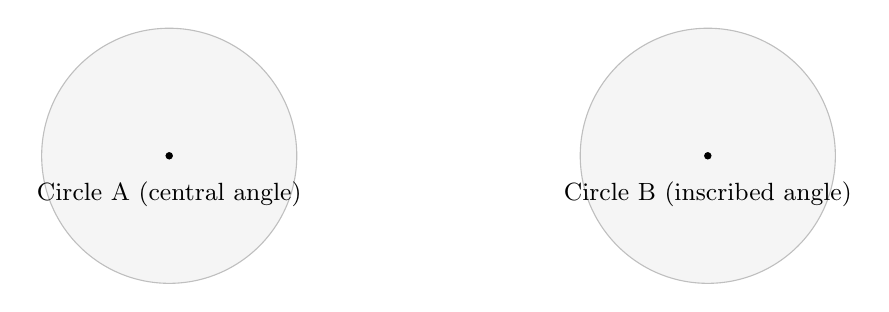
\begin{tikzpicture}[scale=0.9, font=\small]
  \begin{scope}[xshift=-3.8cm]
    \draw[gray!50, fill=gray!8] (0,0) circle (1.8);
    \fill (0,0) circle (1.5pt);
    \node[below, yshift=-6pt] at (0,0) {Circle A (central angle)};
  \end{scope}
  \begin{scope}[xshift=3.8cm]
    \draw[gray!50, fill=gray!8] (0,0) circle (1.8);
    \fill (0,0) circle (1.5pt);
    \node[below, yshift=-6pt] at (0,0) {Circle B (inscribed angle)};
  \end{scope}
\end{tikzpicture}
\end{center}

\textbf{The arc intercepted by an angle} is the arc that lies \blank{5cm} the angle.

\vspace{6pt}
\textbf{Tangent:}

A \textbf{tangent} is a line that touches the circle at exactly \blank{2cm} point (the point of tangency).

At the point of tangency, the tangent is \blank{3.5cm} to the radius. \textit{(We will prove this in Section 4.)}

\textbf{Is a tangent the same as a chord?} \blank{1cm}\quad Explain: \blank{6.5cm}

\vspace{6pt}
\textbf{Naming arcs:}

A \textbf{minor arc} is the \blank{3cm} arc between two points (less than a semicircle).

A \textbf{major arc} is the \blank{3cm} arc (more than a semicircle).

A \textbf{semicircle} is exactly \blank{2.5cm} of the circle --- it is the arc cut by a \blank{3cm}.

\begin{tcolorbox}[retrieval]
\begin{enumerate}[leftmargin=*, itemsep=10pt]
  \item What is the difference between a chord and a diameter? \answerline
  \item What is the difference between a central angle and an inscribed angle? \answerline
  \item In a circle with diameter 14\,cm, what is the radius? \answerline
  \item A tangent line touches a circle at one point. What property does it have relative to the radius at that point? \answerline
  \item \textit{(Stretch)} Can two different chords in the same circle be equal in length? What would this tell you about their distances from the centre? \answerline
\end{enumerate}
\selfcheck
\end{tcolorbox}

\clearpage

% ───────────────────────────────────────────────────
\section{Section 2 --- Chord Properties}

\begin{tcolorbox}[learningtarget]
\small\textit{\textbf{Learning target:} I can apply the two chord properties --- the perpendicular bisector property and the equal chords/equal distance property --- to solve problems.}
\end{tcolorbox}

\subsection{Vocabulary}

\renewcommand{\arraystretch}{1.9}
\begin{tabularx}{\linewidth}{|p{4.2cm}|X|X|}
\hline
\rowcolor{accentlight}\textbf{Term} & \textbf{Definition in your own words} & \textbf{One example} \\
\hline
Perpendicular bisector & & \\ \hline
Bisect               & & \\ \hline
Equidistant          & & \\ \hline
Distance from centre to chord & & \\ \hline
\end{tabularx}
\renewcommand{\arraystretch}{1}

\subsection{Guided Notes}

\textbf{Property 1: The Perpendicular from the Centre Bisects the Chord}

If a line from the \blank{3cm} of a circle is perpendicular to a chord, then it \blank{4.5cm} that chord.

\begin{center}
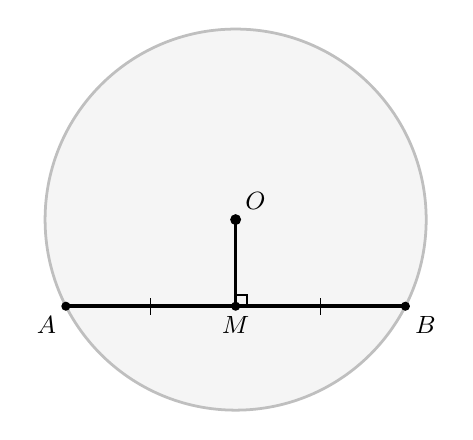
\begin{tikzpicture}[scale=1.1, font=\small]
  % r=2.2, d=1 from centre, half-chord = sqrt(2.2^2-1^2)=sqrt(3.84)=1.96
  \draw[gray!50, fill=gray!8, line width=1pt] (0,0) circle (2.2);
  \fill (0,0) circle (1.8pt);
  \node[above right] at (0,0) {$O$};
  % Chord AB
  \draw[line width=1.3pt] (-1.96,-1) -- (1.96,-1);
  \node[below left]  at (-1.96,-1) {$A$};
  \node[below right] at (1.96,-1)  {$B$};
  \node[below]       at (0,-1)     {$M$};
  \fill (-1.96,-1) circle (1.5pt);
  \fill (1.96,-1)  circle (1.5pt);
  \fill (0,-1)     circle (1.5pt);
  % Perpendicular from O to M
  \draw[line width=1pt] (0,0)--(0,-1);
  % Right-angle mark
  \draw[line width=0.8pt] (0.13,-1)--(0.13,-0.87)--(0,-0.87);
  % Equal tick marks on half-chord
  \draw (-0.98,-1.1)--(-0.98,-0.9);
  \draw ( 0.98,-1.1)--( 0.98,-0.9);
\end{tikzpicture}
\end{center}

In symbols: If $OM \perp AB$, then $AM =$ \blank{2cm}

\textbf{The converse is also true:} If a line from the centre bisects a chord, then it is \blank{3.5cm} to the chord.

\begin{tcolorbox}[worked, title=Worked Example 1]
A chord AB is 16\,cm long. The perpendicular from centre O meets AB at M. Find AM.
\begin{quote}
Since $OM \perp AB$ and passes through the centre, it bisects $AB$.\\
$AM = \blank{2cm}/2 = \blank{2cm}$\,cm
\end{quote}
\textbf{Now extend --- use the Pythagorean theorem.} If the radius is 10\,cm, find OM.
\begin{quote}
Right triangle OMA:\quad $OA = \blank{1.8cm}$ (radius),\quad $AM = \blank{1.8cm}$,\quad $OM = ?$\\[5pt]
$OA^2 = OM^2 + AM^2$\\[3pt]
$10^2 = OM^2 + 8^2$\\[3pt]
$OM^2 = \blank{2cm} - \blank{2cm} = \blank{2cm}$\\[3pt]
$OM = \blank{2cm}$\,cm
\end{quote}
\textbf{Explain:} Which side is the hypotenuse in triangle OMA? How do you know?
\answerline
\end{tcolorbox}

\textbf{Property 2: Equal Chords Are Equidistant from the Centre}

In the same circle:
\begin{itemize}[itemsep=2pt]
  \item If two chords are \blank{3.5cm} in length, then they are \blank{3.5cm} from the centre.
  \item Conversely: if two chords are the same distance from the centre, they are \blank{3.5cm}.
\end{itemize}

\begin{center}
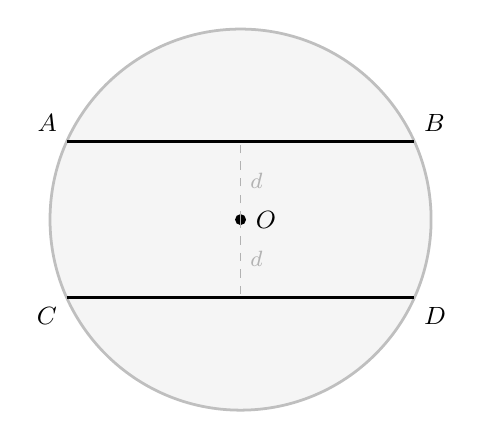
\begin{tikzpicture}[scale=1.1, font=\small]
  % r=2.2, d=0.9
  \draw[gray!50, fill=gray!8, line width=1pt] (0,0) circle (2.2);
  \fill (0,0) circle (1.8pt);
  \node[right, xshift=2pt] at (0,0) {$O$};
  % Half-chord = sqrt(2.2^2-0.9^2)=sqrt(4.84-0.81)=sqrt(4.03)=2.007
  \draw[line width=1.3pt] (-2.007, 0.9) -- (2.007, 0.9);
  \draw[line width=1.3pt] (-2.007,-0.9) -- (2.007,-0.9);
  \node[above left]  at (-2.007, 0.9) {$A$};
  \node[above right] at ( 2.007, 0.9) {$B$};
  \node[below left]  at (-2.007,-0.9) {$C$};
  \node[below right] at ( 2.007,-0.9) {$D$};
  % Distance lines
  \draw[dashed, gray!60] (0,0)--(0, 0.9) node[right, midway, font=\footnotesize] {$d$};
  \draw[dashed, gray!60] (0,0)--(0,-0.9) node[right, midway, font=\footnotesize] {$d$};
\end{tikzpicture}
\end{center}

If $AB = CD$, then $d_1 =$ \blank{2cm}

\begin{tcolorbox}[misconc]
\textbf{Wrong idea:} ``The longest chord should be farthest from the centre.''

\smallskip
\textbf{Why it fails:} It's the opposite. The chord \textit{closest} to the centre is the longest. The diameter --- the longest chord of all --- passes through the centre at distance 0. As a chord moves farther from the centre, it gets shorter and shorter until it disappears at the edge.
\end{tcolorbox}

\begin{tcolorbox}[worked, title=Worked Example 2]
Two chords PQ and RS are each 24\,cm long in a circle with radius 13\,cm.
\begin{quote}
Since $PQ = RS$, they are equidistant from the centre.\\[4pt]
Let M be the midpoint of PQ.\quad $PM = \blank{2cm}/2 = \blank{2cm}$\\[4pt]
Right triangle OMP:\quad $OP = 13$ (radius),\quad $PM = 12$,\quad $OM = ?$\\[4pt]
$13^2 = OM^2 + 12^2 \implies OM = \blank{2cm}$\\[4pt]
Therefore both chords are \blank{2cm}\,cm from the centre.
\end{quote}
\end{tcolorbox}

\begin{tcolorbox}[retrieval]
\begin{enumerate}[leftmargin=*, itemsep=10pt]
  \item State the perpendicular bisector chord property in your own words. \answerline
  \item A chord is 18\,cm long. The perpendicular from the centre has length 12\,cm. Find the radius. (Draw a diagram first.) \answerline\answerline
  \item Two chords in the same circle are both 10\,cm long. What can you conclude about their distances from the centre? \answerline
  \item In a circle with radius 5\,cm, a chord is 3\,cm from the centre. How long is the chord? \answerline
  \item \textit{(Stretch)} A chord is 8\,cm from the centre of a circle with radius 17\,cm. Another chord is 15\,cm from the centre. Which chord is longer? By how much? \answerline
\end{enumerate}
\selfcheck
\end{tcolorbox}

\begin{tcolorbox}[connection]
\small\textbf{Connection:} The perpendicular bisector of a chord passes through the centre. You can use this to find the centre of any circle if you don't know where it is. How would you do that if given only the circle drawn on paper? Describe the steps.
\answerline\answerline
\end{tcolorbox}

\clearpage

% ───────────────────────────────────────────────────
\section{Section 3 --- Central Angle and Inscribed Angle Theorem}

\begin{tcolorbox}[learningtarget]
\small\textit{\textbf{Learning target:} I can apply the inscribed angle theorem to find unknown angles, and explain why inscribed angles subtending the same arc are equal.}
\end{tcolorbox}

\subsection{Vocabulary}

\renewcommand{\arraystretch}{1.9}
\begin{tabularx}{\linewidth}{|p{4.2cm}|X|X|}
\hline
\rowcolor{accentlight}\textbf{Term} & \textbf{Definition in your own words} & \textbf{One example} \\
\hline
Inscribed angle theorem & & \\ \hline
Subtend                 & & \\ \hline
Same arc                & & \\ \hline
\end{tabularx}
\renewcommand{\arraystretch}{1}

\subsection{Guided Notes}

\textbf{The Inscribed Angle Theorem:}

The inscribed angle is \blank{5cm} the central angle that subtends the same arc.

\[\text{Inscribed angle} = \tfrac{1}{2} \times \text{Central angle}
  \qquad\text{OR}\qquad
  \text{Central angle} = \underline{\phantom{XX}} \times \text{Inscribed angle}\]

\begin{center}
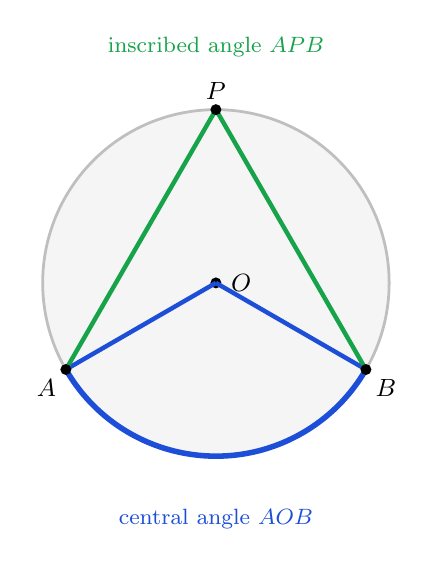
\begin{tikzpicture}[scale=1.1, font=\small]
  % A at 210, B at 330, P at 90, O at centre
  \coordinate (O) at (0,0);
  \coordinate (A) at ({cos(210)*2},{sin(210)*2});
  \coordinate (B) at ({cos(330)*2},{sin(330)*2});
  \coordinate (P) at (0,2);
  \draw[gray!50, fill=gray!8, line width=1pt] (O) circle (2);
  \fill (O) circle (1.8pt); \node[right, xshift=2pt] at (O) {$O$};
  % Central angle (blue)
  \draw[dblue, line width=1.6pt] (O)--(A);
  \draw[dblue, line width=1.6pt] (O)--(B);
  \draw[dblue, line width=2pt] (A) arc (210:330:2);
  % Inscribed angle (green)
  \draw[accent, line width=1.6pt] (P)--(A);
  \draw[accent, line width=1.6pt] (P)--(B);
  % Points
  \fill (A) circle (1.8pt); \node[below left]  at (A) {$A$};
  \fill (B) circle (1.8pt); \node[below right] at (B) {$B$};
  \fill (P) circle (1.8pt); \node[above]        at (P) {$P$};
  % Labels
  \node[dblue,  below]  at (0,-2.5) {\footnotesize central angle $AOB$};
  \node[accent, above] at (0, 2.5) {\footnotesize inscribed angle $APB$};
\end{tikzpicture}
\end{center}

Angle $AOB$ (central) $=$ \blank{2cm}\dgr{}\qquad
Angle $APB$ (inscribed, same arc $AB$) $=$ \blank{2cm}\dgr{}

\begin{tcolorbox}[worked, title=Worked Example 1]
Central angle $AOB = 80\dgr{}$. Find inscribed angle $APB$ subtending the same arc.
\begin{quote}
Inscribed angle $= 80\dgr{} \div \blank{1.5cm} = \blank{1.5cm}\dgr{}$
\end{quote}
\end{tcolorbox}

\begin{tcolorbox}[worked, title=Worked Example 2]
Inscribed angle $APB = 35\dgr{}$. Find central angle $AOB$ subtending the same arc.
\begin{quote}
Central angle $= 2 \times 35\dgr{} = \blank{1.5cm}\dgr{}$
\end{quote}
\end{tcolorbox}

\textbf{Explain:} Why does being at the centre make the central angle ``see'' the arc at twice the angle?
\answerline\answerline

\textbf{Corollary: Inscribed angles subtending the same arc are equal.}

$APB = AQB = \tfrac{1}{2} \times AOB$\quad regardless of where P and Q are on the major arc.

\begin{tcolorbox}[misconc]
\textbf{Wrong idea:} ``Any angle drawn inside a circle is 90\dgr{}.''

\smallskip
\textbf{Why it fails:} Only inscribed angles that subtend a \textit{diameter} equal 90\dgr{}. That is a special case. The special case: when $AB$ is a diameter, $AOB = 180\dgr{}$, so the inscribed angle $= 180\dgr{}/2 = \blank{1.5cm}\dgr{}$.
\end{tcolorbox}

\textbf{Angles in a semicircle:}

If $AB$ is a diameter, then any inscribed angle $APB = \blank{1.5cm}\dgr{}$.

\vspace{6pt}
\textbf{Finding unknown angles:}

In a circle, central angle $AOB = 110\dgr{}$. Find:

a) Inscribed angle $APB$ (same arc) $= \blank{2cm}\dgr{}$

b) Inscribed angle $AQB$ subtending the \textbf{major} arc $AB$.\\
\quad\textit{(Hint: major arc central angle $= 360\dgr{} - 110\dgr{} = \blank{2cm}\dgr{}$)}\quad
$AQB = \blank{2cm}\dgr{}/2 = \blank{2cm}\dgr{}$

\begin{tcolorbox}[retrieval]
\begin{enumerate}[leftmargin=*, itemsep=10pt]
  \item State the inscribed angle theorem in your own words. \answerline
  \item A central angle is 144\dgr{}. What is the inscribed angle subtending the same arc? \answerline
  \item An inscribed angle is 23\dgr{}. What is the central angle subtending the same arc? \answerline
  \item Why do all inscribed angles subtending the same arc equal each other? \answerline
  \item \textit{(Stretch)} Arc CD has central angle 130\dgr{}. Find inscribed angle CPD. \answerline
\end{enumerate}
\selfcheck
\end{tcolorbox}

\clearpage

% ───────────────────────────────────────────────────
\section{Section 4 --- Tangent-Radius Property}

\begin{tcolorbox}[learningtarget]
\small\textit{\textbf{Learning target:} I can apply the tangent-radius perpendicularity property and use it with the Pythagorean theorem to solve problems.}
\end{tcolorbox}

\subsection{Vocabulary}

\renewcommand{\arraystretch}{1.9}
\begin{tabularx}{\linewidth}{|p{4.8cm}|X|X|}
\hline
\rowcolor{accentlight}\textbf{Term} & \textbf{Definition in your own words} & \textbf{One example} \\
\hline
Tangent                    & & \\ \hline
Point of tangency          & & \\ \hline
Perpendicular              & & \\ \hline
Tangent from external point & & \\ \hline
\end{tabularx}
\renewcommand{\arraystretch}{1}

\subsection{Guided Notes}

\textbf{Tangent-Radius Property:}

A tangent to a circle is \blank{5cm} to the radius at the point of tangency.

\begin{center}
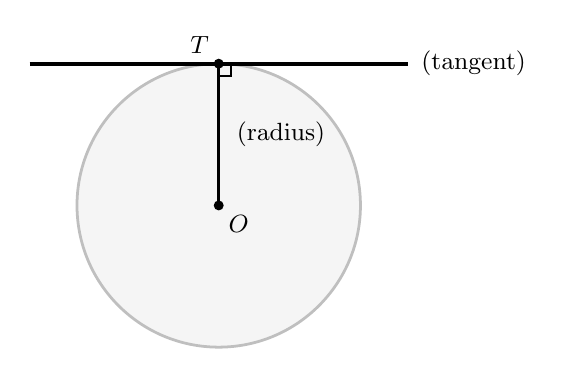
\begin{tikzpicture}[scale=1.0, font=\small]
  \draw[gray!50, fill=gray!8, line width=1pt] (0,0) circle (1.8);
  \fill (0,0) circle (1.8pt); \node[below right] at (0,0) {$O$};
  \coordinate (T) at (0,1.8);
  \draw[line width=1.5pt] (-2.4,1.8) -- (2.4,1.8);
  \draw[line width=0.8pt] (0.16,1.8)--(0.16,1.64)--(0,1.64);
  \draw[line width=1pt] (0,0)--(0,1.8);
  \fill (T) circle (1.8pt); \node[above left] at (T) {$T$};
  \node[right] at (2.45,1.8) {(tangent)};
  \node[right, xshift=3pt] at (0,0.9) {(radius)};
\end{tikzpicture}
\end{center}

Angle $OTP = $ \blank{2cm}\dgr{}

This means: if you know a line is tangent, the angle at the point of tangency is automatically \blank{3.5cm}.

\begin{tcolorbox}[worked, title=Worked Example]
A tangent PT touches a circle with centre O and radius 5\,cm. Point P is 13\,cm from the centre. Find PT.

\begin{center}
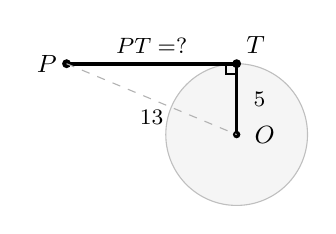
\begin{tikzpicture}[scale=0.9, font=\small]
  % T at top of circle, O below, P level with T
  % OT is vertical, PT is horizontal → right angle at T is geometrically exact
  % Proportions: OT=1 (=5 cm), PT=2.4 (=12 cm), PO=2.6 (=13 cm)
  \coordinate (O) at (0,-1);
  \coordinate (T) at (0, 0);
  \coordinate (P) at (-2.4, 0);
  \draw[gray!50, fill=gray!8] (O) circle (1);
  \fill (O) circle (1.5pt); \node[right, xshift=3pt] at (O) {$O$};
  \fill (T) circle (1.8pt); \node[above right] at (T) {$T$};
  \fill (P) circle (1.8pt); \node[left] at (P) {$P$};
  \draw[line width=1.5pt] (P)--(T);           % tangent segment (horizontal)
  \draw[line width=1pt]   (O)--(T);           % radius (vertical)
  \draw[dashed, gray!60]  (P)--(O);           % hypotenuse PO
  % Right-angle mark at T
  \draw[line width=0.8pt] (-0.15,0)--(-0.15,-0.15)--(0,-0.15);
  \node[right, font=\footnotesize] at (0.1,-0.5) {5};
  \node[below, font=\footnotesize] at (-1.2,-0.52) {13};
  \node[above, font=\footnotesize] at (-1.2, 0)  {$PT=?$};
\end{tikzpicture}
\end{center}

\begin{quote}
Right angle at \blank{1.5cm} (tangent $\perp$ radius)\quad Hypotenuse $= PO = \blank{1.5cm}$\\[5pt]
$PT^2 = PO^2 - OT^2 = 13^2 - 5^2 = \blank{2cm} - \blank{2cm} = \blank{2cm}$\\[3pt]
$PT = \blank{2cm}$\,cm
\end{quote}
\textbf{Explain:} Why is $PO$ the hypotenuse?
\answerline
\end{tcolorbox}

\textbf{Equal tangents from an external point:}

From any external point P, two tangents can be drawn to a circle. The two tangent segments are \blank{4cm} in length.

$PT_1 = $ \blank{2cm}

\begin{tcolorbox}[connection]
\small\textbf{Alberta context:} A circular fountain in a Calgary park has radius 3\,m. A path runs tangent to the fountain, and the nearest point on the path is 5\,m from the fountain's centre. How long is the section of path from where it first touches the tangent line to where it last could touch? \textit{(Hint: find the tangent length, then consider symmetry.)}
\answerline
\end{tcolorbox}

\begin{tcolorbox}[retrieval]
\begin{enumerate}[leftmargin=*, itemsep=10pt]
  \item State the tangent-radius property. \answerline
  \item A tangent is drawn to a circle of radius 6\,cm. The external point is 10\,cm from the centre. Find the tangent length. \answerline
  \item From an external point P, two tangents are drawn. One segment is 8\,cm. What is the length of the other? \answerline
  \item Why does the tangent-radius property create a right triangle? How is this useful? \answerline
  \item \textit{(Stretch)} Circle with centre O, radius 7\,cm. Tangent at T, external point P where $OP = 25$\,cm. Find PT. Then find angle OPT to the nearest degree. \answerline
\end{enumerate}
\selfcheck
\end{tcolorbox}

\clearpage

% ───────────────────────────────────────────────────
\section*{Unit Synthesis}

\textit{Fill this in from memory. Notes closed.}

\subsection*{Part A --- Key ideas}

\begin{enumerate}[leftmargin=*, itemsep=10pt]
  \item State the two chord properties from Section 2.
  \answerline\answerline
  \item State the inscribed angle theorem. What is the special case when the chord is a diameter?
  \answerline\answerline
  \item State the tangent-radius property. How does it allow you to use the Pythagorean theorem?
  \answerline\answerline
\end{enumerate}

\subsection*{Part B --- Practise from memory}

In a circle with centre O and radius 10\,cm: chord $AB = 16$\,cm, inscribed angle $APB = 38\dgr{}$.

Find:\quad a) the distance from O to chord AB.\quad b) the central angle AOB.

Show working:
\answerline\answerline\answerline

\subsection*{Part C --- Go back to your Pre-Knowledge Check}

Read what you wrote before this unit started.

\begin{enumerate}[leftmargin=*, itemsep=10pt]
  \item How many circle parts did you label correctly? Which ones did you not know? \answerline
  \item What is an inscribed angle? How does it compare to your guess? \answerline\answerline
\end{enumerate}

\vfill
\begin{center}
  \color{slatelight}\textit{End of Circle Geometry Notes Package.}
\end{center}

\end{document}
